\documentclass[../main.tex]{subfiles}

\begin{document}

\section{Channel coding}

One of the first uses of coding theory and error-correcting codes was in the transmission of information over an unreliable channel. In this section we give a motivation for some of the concepts in coding theory that will be used throughout the course. The main reference for this section is \cite[Chapter 2]{ling2004coding}.

\subsection{Communication channels}

We can think of a communication channel as a randomized transformation of an input $x \in \mathcal{X}$ to an output $y \in \mathcal{Y}$. The channel is described by the input and output \emph{alphabets} $\mathcal{X}$ and $\mathcal{Y}$ as well as the \emph{transition probabilities} $\P[y \mid x]$ for all $x \in \mathcal{X}$ and $y \in \mathcal{Y}$ (or the probability density function $p(y \mid x)$). The idea is that the transmitted symbol $x$ is received with some random error as the symbol $y$.

Communication channels can be for example an antenna transmitting electromagnetic waves to send a message to a receiver, or a physical medium such as a transistor storing information that can be accessed at a later point in time.

\begin{example}
One of the simplest channels is the \emph{binary symmetric channel (BSC)} which has alphabets $\mathcal{X} = \mathcal{Y} = \{0, 1\}$ and transition probabilities
\begin{align*}
    \P[y = 0 \mid x = 0] = \P[y = 1 \mid x = 1] &= 1 - p \\
    \P[y = 0 \mid x = 1] = \P[y = 1 \mid x = 0] &= p.
\end{align*}
Here, $p \in [0, 1]$ is known as the \emph{crossover probability}. Sending one bit (= element of $\{0, 1\}$) through this channel results in a probability $p$ of receiving the bit in error. Even in a good channel, the error probability may be too large as we want the error probability to be as close to zero as possible.
\end{example}

The key solution to this problem is to use the channel many times to send just one bit. Let's use the channel 3 times by repeating the desired bit value, \ie, instead of $0$ send $000$ and instead of $1$ send $111$. The receiver should do majority voting on the output (choose the bit that appears the most). If they receive $010$ decode to $0$ and if they receive $110$ decode to $1$. This method produces the correct result if the channel produces 1 or fewer errors. Therefore, assuming that the errors are independent on the 3 different uses of the channel (the channel is said to be \emph{memoryless}), then the new error probability is
\begin{equation*}
    P_e = \underbrace{\binom{3}{3}p^3}_{\text{probability of 3 errors}} + \underbrace{\binom{3}{2}p^2 (1 - p)}_{\text{probability of 2 errors}} = 3p^2 - 2p^3,
\end{equation*}
which is usually much smaller than $p$. In general, we may repeat the message $2r + 1$ times such that as long as $\leq r$ errors are introduced, it is still possible to decode the correct answer. Such a coding scheme is known as a repetition code. We are able to send 1 bit by using the channel $n = 2r + 1$ times, which means that the communication rate is $1 / n$.

By using the channel many times, we have created a new channel on the alphabets $\mathcal{X}^n$ and $\mathcal{Y}^n$ with some new transition probabilities. If $n$ is fixed, then we want to send messages from a proper subset $\mathcal{C} \subset \mathcal{X}^n$. The subset $\mathcal{C}$ is known as a block code of length $n$.

\subsection{Block codes}

Let $\Sigma$ be a finite set of size $q = \lvert \Sigma \rvert$, known as the alphabet. We denote $\Sigma^n = \Sigma \times \dots  \times \Sigma$ to be the set of $n$-tuples (also known as \emph{words}) with entries in $\Sigma$. A nonempty subset $\mathcal{C} \subset \Sigma^n$ is said to be a \emph{block code}\footnote{The word block refers to the fact that the codewords all have the same length $n$. There are also codes of variable length and codes where the different symbols are in different alphabets.} of \emph{length} $n$ over the alphabet $\Sigma$. The set is also known as the \emph{codebook} and the elements as \emph{codewords}. The \emph{size} of a code $\mathcal{C}$ is $M = \lvert \mathcal{C} \rvert$ and the \emph{rate} of a code is $\mathcal{R} = \log_q(M) / n$. The rate describes the relative size of the code in the ambient space $\Sigma^n$. With these notations we say that $\mathcal{C}$ is an $(n, M)_q$-code.

\begin{example}
Above we considered the block code $\mathcal{C} = \{000, 111\} \subseteq \{0, 1\}^3$ of length $n = 3$ and size $M = 2$ over an alphabet of size $q = 2$. We say that $\mathcal{C}$ is an $(3, 2)_2$-code. The rate of this code is $\mathcal{R} = \log_2(2) / 3 = 1 / 3$, which matches the communication rate discussed above.
\end{example}

When we send information using a block code, we encode each of the $M$ possible messages as one of the codewords and send that through the product channel by using the channel $n$ times. The flow of this process can be seen in Figure~\ref{fig:channel_coding}.

\begin{figure}
    \centering
    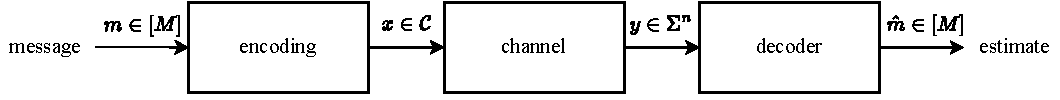
\includegraphics[width=.9\textwidth]{images/channel_coding_diagram.pdf}
    \caption{The flow of a message going through a communication channel with encoding and decoding}
    \label{fig:channel_coding}
\end{figure}

Given the transition probabilities of the communication channel, we may compute the probabilities of the word $y$ being received given that a specific word $x$ was sent as $\P[y \mid x]$. As we only send codewords in $\mathcal{C}$, we are considering the likelihoods $\P[y \mid x]$ for all $x \in \mathcal{C}$. In \emph{maximum likelihood (ML) decoding}, we choose the codeword $x \in \mathcal{C}$ that maximizes this likelihood for the given output $y$, \ie, the decoder outputs\footnote{There has to be some rule for breaking a tie in case there are many codewords that maximize the likelihood function, but this is not important for now.}
\begin{equation*}
    \hat{x} = \argmax_{x \in \mathcal{C}} \P[y \mid x].
\end{equation*}

\begin{example}
Consider the ($n$-fold) binary symmetric channel with crossover probability $p < \frac{1}{2}$. Let $x \in \mathcal{C}$ be a codeword and $y \in \{0, 1\}^n$ the received word. Let
\begin{equation*}
    d = \lvert \{i \in [n] \colon x_i \neq y_i \} \rvert
\end{equation*}
to be the number of coordinates where $x$ and $y$ differ. Then,
\begin{equation*}
    \P[y \mid x] = p^d (1 - p)^{n - d} = \underbrace{(1 - p)^n}_{\text{independent of $x$ and $y$}} \left( \frac{p}{1 - p} \right)^d
\end{equation*}
as the errors are independent in each of the coordinates. Denote $d = d(x, y)$. Then
\begin{equation*}
    \hat{x} = \argmax_{x \in \mathcal{C}} \P[y \mid x] = \argmax_{x \in \mathcal{C}} \left( \frac{p}{1 - p} \right)^{d(x, y)} = \argmin_{x \in \mathcal{C}} d(x, y).
\end{equation*}
The above is due to the fact that $\frac{p}{1 - p} < 1$, so the quantity is maximized with the smallest exponent.
\end{example}

According to the example above, ML decoding on the binary symmetric channel is equivalent to minimizing the distance given by $d(x, y)$. That is, given the output $y$, find the codeword $x \in \mathcal{C}$ that is closest to $y$ in the distance given by $d(x, y)$.

\subsection{Hamming distance}

For $x, y \in \Sigma^n$, the \emph{Hamming distance} between $x$ and $y$ is given by
\begin{equation*}
    d(x, y) = \lvert \{ i \in [n] \colon x_i \neq y_i \} \rvert.
\end{equation*}
The Hamming distance has the following properties:
\begin{itemize}
    \item $0 \leq d(x, y) \leq n$ for all $x, y \in \Sigma^n$,
    \item $d(x, y) = 0$ if and only if $x = y$,
    \item $d(x, y) = d(y, x)$ for all $x, y \in \Sigma^n$, and
    \item $d(x, z) \leq d(x, y) + d(y, z)$ for all $x, y, z \in \Sigma^n$ (triangle inequality).
\end{itemize}

We can also write $d(x, y) = d(x_1, y_1) + \dots + d(x_n, y_n)$, where
\begin{equation*}
    d(x_i, y_i) = \begin{dcases*}
        1 & if $x_i \neq y_i$ \\
        0 & if $x_i = y_i$
    \end{dcases*}.
\end{equation*}
To prove the triangle inequality it is enough to show it for just $d(x_i, z_i)$. If $d(x_i, y_i) = 0$, then the inequality is clear. On the other hand, if $d(x_i, z_i) = 1$, then $x_i \neq z_i$, so either $x_i \neq y_i$ or $y_i \neq z_i$. Hence, $d(x_i, y_i) + d(y_i, z_i) \geq 1 = d(x_i, z_i)$.

In general, we may use \emph{minimum distance decoding} by using the rule
\begin{equation*}
    \hat{x} = \argmin_{x \in \mathcal{C}} d(x, y).
\end{equation*}
This may or may not be equivalent to ML decoding depending on the channel.

It is usually the case that the output $y$ of a channel is close to the input $x$ in the Hamming distance. Therefore, the minimum distance decoding rule makes an error whenever the output $y$ of the channel is closer to another codeword $x' \neq x \in \mathcal{C}$ than to the originally sent codeword~$x$. Therefore, we want the codewords in $\mathcal{C}$ to be far away from each other so that the error probability of the minimum distance decoding algorithm is low\footnote{The minimum distance is not the only factor that determines the error-correction performance of a code.}.

The \emph{minimum distance} of a block code $\mathcal{C} \subset \Sigma^n$ is defined as
\begin{equation*}
    d(\mathcal{C}) = \min \{d(x, y) \colon x, y \in \mathcal{C}, x \neq y\}.
\end{equation*}
Further, if $\mathcal{C}$ contains just one element, then we set $d(\mathcal{C}) = n + 1$ (sometimes also $d(\mathcal{C}) = \infty$). If $\mathcal{C} \subset \Sigma^n$ has $M$ elements and minimum distance $d$, then we say that $\mathcal{C}$ is an $(n, M, d)$-code.

\begin{lemma}
If $y \in \Sigma^n$ and $2v < d(\mathcal{C})$, then there is at most one $x \in \mathcal{C}$ such that $d(x, y) \leq v$.
\end{lemma}

\begin{proof}
Assume that there are $x, x' \in \mathcal{C}$ such that $d(x, y) \leq v$ and $d(x', y) \leq v$. Then, $d(x, x') \leq d(x, v) + d(v, x') \leq 2v < d(\mathcal{C})$, so $x = x'$.
\end{proof}

If the codeword $x \in \mathcal{C}$ is sent and the word $y \in \Sigma^n$ is received such that $d(x, y) \leq v$ with $2v < d(\mathcal{C})$, then $x \in \mathcal{C}$ is the unique codeword closest to $y$. Thus, the minimum distance decoding algorithm will make the correct decision. In particular, we say that $\mathcal{C}$ is \emph{$v$-error-correcting}. The value $t = \lfloor (d(\mathcal{C}) - 1) / 2 \rfloor$ is said to be the \emph{unique decoding radius}.

% Before correcting any transmission errors, it is important to be able to tell if an error has occurred in the first place. We say that a code is $u$-error-detecting if changing a codeword in at most $u$ coordinates results in a word not in the code. Similarly, we say that a code is $v$-error-correcting, if changing distinct codewords $x \neq y$ in at most $v$ coordinates always results in different words.

% In some applications of coding theory, we may think of an adversary that is corrupting the words instead of random errors form the channel. In this setting we may assume that the adversary has limited power and is only able to corrupt a limited number of coordinates. In these situations we want to know how many errors we can detect and correct.

% \begin{lemma}\label{lem:error_detection}
% A code $\mathcal{C}$ is $u$-error-detecting if and only if $d(\mathcal{C}) \geq u + 1$.
% \end{lemma}

% \begin{proof}
% \ProofLeftarrow Let $d(\mathcal{C}) \geq u + 1$ and let $x \in \mathcal{C}$ be a codeword. If $z \in \Sigma^n$ is a word such that $z \neq x$ and $d(x, z) \leq u < d(\mathcal{C})$, then $z \notin \mathcal{C}$, so $\mathcal{C}$ is $u$-error-detecting.

% \ProofRightarrow From the definition of $u$-error-detecting it is clear that if $x \in \mathcal{C}$ is a codeword, then there does not exist another codeword $y \neq x$ such that $d(x, y) \leq u$. Thus, $d(\mathcal{C}) \geq u + 1$.
% \end{proof}

% \begin{lemma}
% A code $\mathcal{C}$ is $v$-error-correcting if and only if $d(\mathcal{C}) \geq 2v + 1$.
% \end{lemma}

% \begin{proof}
% Let $x, y$ be words. Then there exists a word $z$ such that $d(x, z), d(y, z) \leq v$ if and only if $d(x, y) \leq 2v$.

% \ProofLeftarrow Let $d(\mathcal{C}) \geq 2v + 1$ and let $x, y \in \mathcal{C}$ be distinct codewords. Then, $d(x, y) \geq d(\mathcal{C}) = 2v + 1$, so there does not exist a word $z$ such that $d(x, z), d(y, z) \leq v$, so $\mathcal{C}$ is $v$-error-correcting.

% \ProofRightarrow Let $x, y \in \mathcal{C}$ be distinct codewords. From the definition of $v$-error-correcting, there does not exist a word $z$ such that $d(x, z), d(y, z) \leq v$, so $d(x, y) \geq 2v + 1$. Therefore, $d(\mathcal{C}) \geq 2v + 1$.
% \end{proof}

% When we say that a code is error-detecting or error-correcting, we only mean that there is in principle a way of finding the closest codeword in a certain radius, not that there is an efficient way of doing that. A large part of coding theory research is finding algorithms to efficiently correct errors in a code.

% \begin{example}
% Let $\mathcal{C} \subset \{0, 1\}^n$ consist of those words that have an even number of $1$'s. Then, any two distinct codewords must differ in at least 2 places, so the minimum distance of $\mathcal{C}$ is 2. Furthermore, changing any coordinate of a codeword will result in a new word with an odd number of $1$'s meaning that it is not a codeword. Thus, $\mathcal{C}$ is $1$-error-detecting.
% \end{example}

A sequence of codes $\mathcal{C}^{(n)} \subset \Sigma^n$ of rate $R$ have $q^{Rn}$ codewords, which grows exponentially in $n$. Even to describe such a set is impractical without any additional structure. It is typical in coding theory to only consider codes with a vector space structure over the alphabet, so that the code can be described in terms of a basis. To do this we will need to understand finite fields and vector spaces over these fields.

\end{document}